\documentclass[twoside,11pt]{article}

\usepackage[utf8]{inputenc}
\usepackage[T1]{fontenc}
\usepackage[ngerman]{babel}
\usepackage{graphicx,curves,float,rotating}
\usepackage[usenames,dvipsnames,svgnames,table]{xcolor}
\usepackage{latexsym,amsmath,amssymb}
\usepackage{a4,amsmath}
\usepackage{hyperref}
\usepackage{theorem}
\usepackage{dcolumn}
\usepackage{fancyhdr}
\usepackage{extramarks}
\usepackage{sectsty}
\usepackage[light]{roboto}

\newcommand{\Frac}[2]{\frac{\displaystyle #1}{\displaystyle #2}}
\newlength{\textwd}
\newlength{\oddsidemargintmp}
\newlength{\evensidemargintmp}
\newcommand{\hspaceof}[2]{\settowidth{\textwd}{#1}\mbox{\hspace{#2\textwd}}}
\newlength{\textht}
\newcommand{\vspaceof}[3]{\settoheight{\textht}{#1}\mbox{\raisebox{#2\textht}{#3}}}
\newcommand{\PreserveBackslash}[1]{\let\temp=\\#1\let\\=\temp}

\newenvironment{deflist}[1][\quad]%
{  \begin{list}{}{%
	\renewcommand{\makelabel}[1]{\textbf{##1}\hfil}%
	\settowidth{\labelwidth}{\textbf{#1}}%
	\setlength{\leftmargin}{\labelwidth}
	\addtolength{\leftmargin}{\labelsep}}}
{  \end{list}}

\newenvironment{Quote}% Definition of Quote
{  \begin{list}{}{%
	\setlength{\rightmargin}{0pt}}
	\item[]\ignorespaces}
{\unskip\end{list}}

\newtheorem{Cor}{Corollary}
\theoremstyle{break}
\theorembodyfont{\itshape}
\newtheorem{Def}[Cor]{Definition}
\theoremheaderfont{\scshape}

\renewcommand{\arraystretch}{1.5}

\newcolumntype{.}{D{.}{.}{-1}}

\textwidth 15cm
\textheight 21.5cm
\oddsidemargin 1cm
\evensidemargin 0cm

% Colors:
\definecolor{blau}{HTML}{355FB3}
\definecolor{rot}{HTML}{B33535}
\definecolor{gruen}{HTML}{3BB335}

%Fonts:
\renewcommand{\rmdefault}{ppl}
\sectionfont{\sffamily\mdseries\textrmlf\LARGE\color{blau}}

% Header:
\fancyhf{}
\fancyhead[EL,OR]{\sffamily{\thepage}}
\fancyhead[OL,ER]{\nouppercase{\sffamily{\firstleftmark}}}
\fancyfoot[OR]{
\includegraphics[width=0.35cm]{./assets/ubpBlue.pdf}}

\begin{document}

% Titelseite:
\pagestyle{empty}

\begin{center}
	\sffamily
    Universität Paderborn \\
    Institut für Informatik \\
    Prof.\ Dr.\ Stefan Böttcher\\[2ex]
    \Large Proseminar Datenkompression – WS 2016/2017

	\vspace*{\fill}
	\Huge \textcolor{blau}{Linear-Time Suffix-Sorting} \\[1ex]
    \LARGE Clemens Damke \\[1ex]
    \Large Matrikelnummer 7011488
	\vspace*{\fill}
\end{center}

\newpage
\
\newpage

% Inhaltsverzeichnis:
\pagestyle{fancy}
\tableofcontents

\newpage
\pagestyle{empty}
\
\newpage
\pagestyle{fancy}

\section{Problemstellung}

Diese Proseminar-Arbeit beschreibt den GSACA-Algorithmus. Hierbei handelt es sich um den ersten rekursionsfreien Linearzeitalgorithmus zur Konstruktion von Suffix-Arrays. \\

Im Folgenden wird zunächst erörtert, was Suffix-Arrays sind und wozu sie benutzt werden.

\subsection{Was ist ein Suffix-Array?}

Das Suffix-Array $SA$ einer Zeichenkette $S$ ist definiert als die lexiographisch aufsteigend sortierte Folge aller Suffixe von $S$.

\begin{figure}[h]
	\centering
	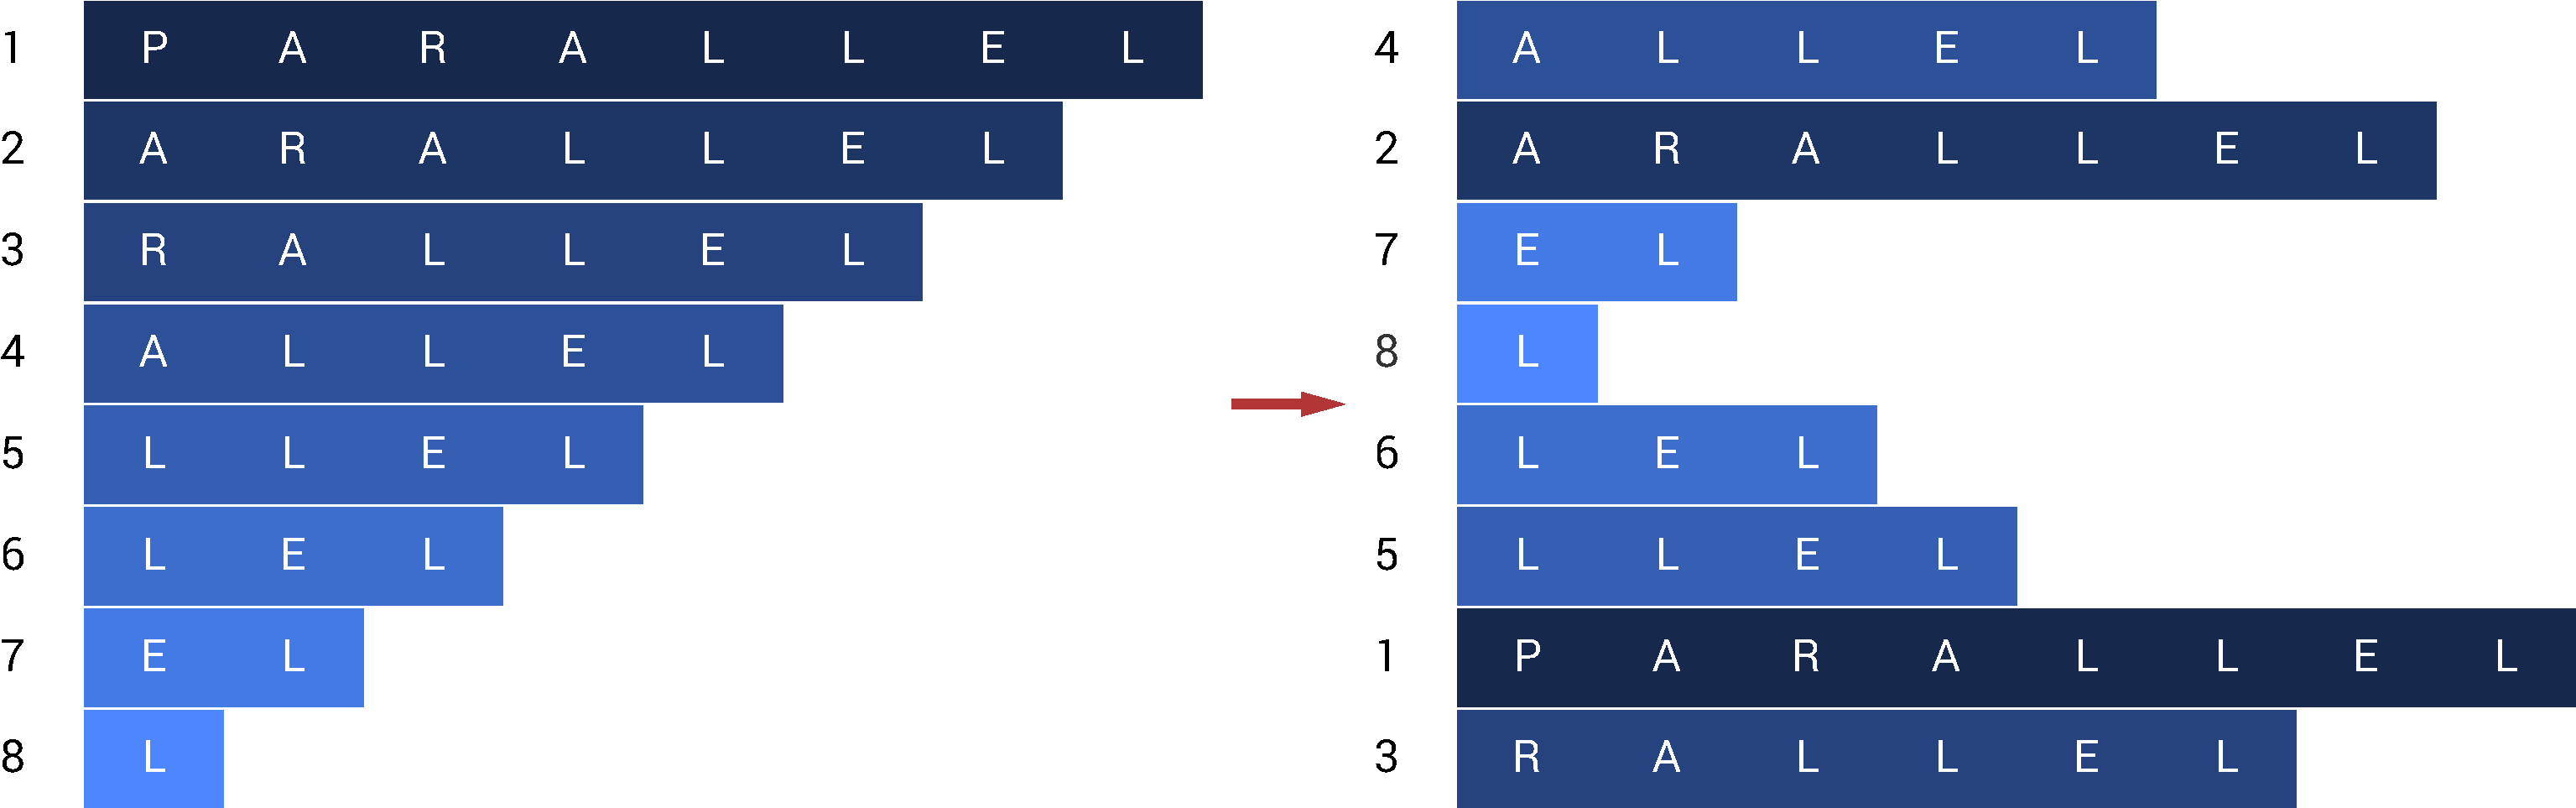
\includegraphics[width=\linewidth,bb=0 0 1474 462]{./assets/whatIsASuffixArray.pdf}
	\caption{Suffixarray für $S =$ `parallel'}
\label{fig:whatIsASuffixArray}
\end{figure}

Um Speicher zu sparen wird $SA$ allerdings nicht als Folge der Suffix-Zeichenketten, sondern als Folge der Startpunkte der Suffixe repräsentiert. Für $S =$ `parallel' wäre also $SA = (4, 2, 7, 8, 6, 5, 1, 3)$. Formal bedeutet dies:
\begin{align*}
	\Sigma &:= \text{streng total geordnetes endliches Alphabet} \\
	S &:= \text{Eingabezeichenkette} = (S[1], \dots, S[n]) \in \Sigma^n, |S| := n \in \mathbb{N} \\
	S[i .. j + 1) = S[i .. j] &:= (S[i], \dots, S[j]) \\
	S_i &:= S[i .. n] \\
	S \sqsubseteq T &:\Leftrightarrow S = T[1 .. |S|] \\
	S <_{lex} T &:\Leftrightarrow (\exists\ i: S[i] < T[i] \land S[1 .. i) = T[1 .. i)) \lor (|S| < |T| \land S \sqsubseteq T) \\
	SA &:= \text{Permutation von } \{1, \dots, |S|\} \text{, sodass } \forall\ i < j: S_{SA[i]} <_{lex} S_{SA[j]}
\end{align*}

\subsection{Einsatzgebiete von Suffix-Arrays}

Suffix-Arrays finden in vielen Bereichen als Index-Datenstruktur Verwendung. Ein typisches Problem, dessen Lösung durch Suffix-Arrays beschleunigt werden kann, ist z.~B. die Substringsuche. Bei dieser soll bestimmt werden, \textit{ob} und wenn ja, \textit{wo} in einem Text $T$ ein Pattern $P$ vorkommt. Ohne einen Index benötigt dieses Problem z.~B. mit Knuth-Morris-Pratt $\mathcal{O}(|T| + |P|)$. Mit einem Suffix-Array als Index über $T$ hingegen lassen sich Matches durch eine binäre Suche in $\mathcal{O}(|P| \log |T|)$ finden. Da i.~d.~R. $|P| \ll |T|$, ist dies ein deutlicher Speedup, welcher z.~B. in Datenbanksystemen für Volltextsuchen und in der Bioinformatik für das Suchen in DNA-Daten nützlich ist.

\begin{figure}[h]
	\centering
	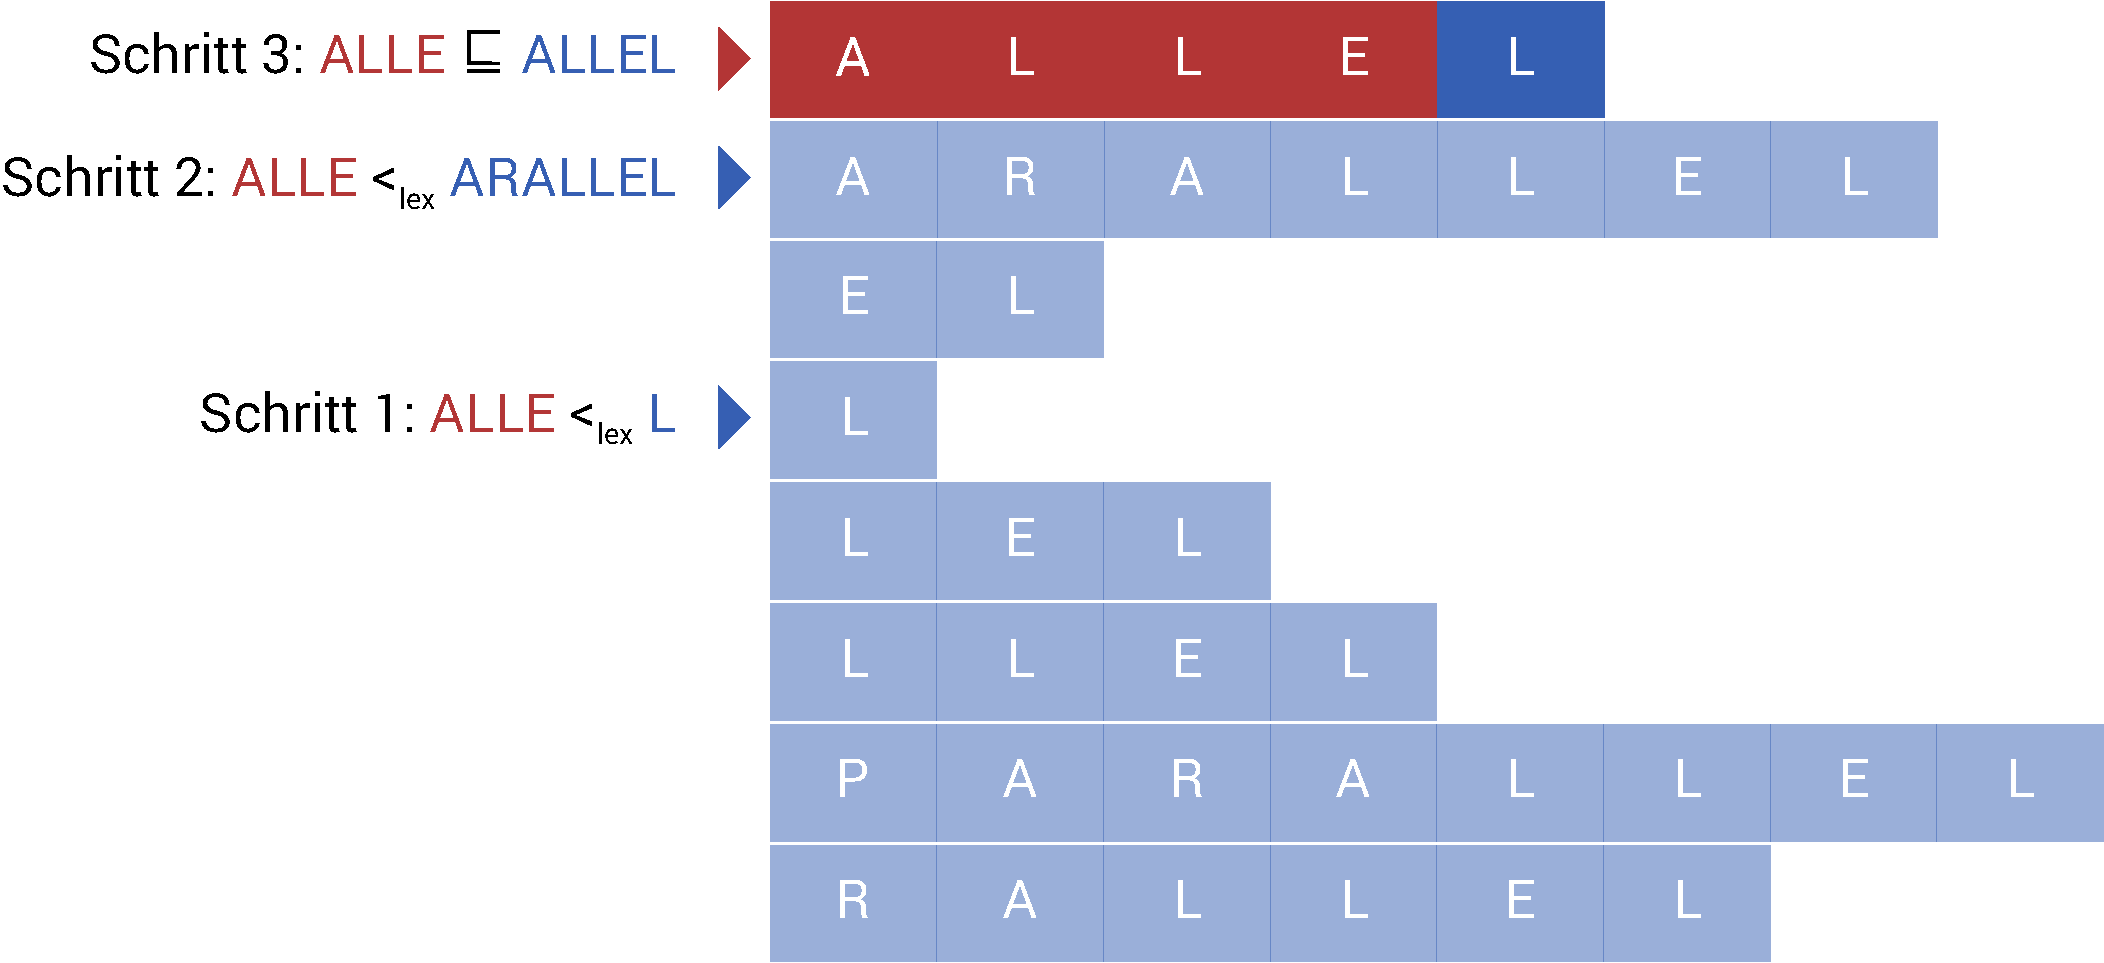
\includegraphics[width=0.7\linewidth,bb=0 0 1010 462]{./assets/substringSearch.pdf}
	\caption{Substringsuche mit $P =$ `alle' und $T =$ `parallel'}
\label{fig:substringSearch}
\end{figure}

Ein weiteres Einsatzgebiet für Suffix-Arrays ist als Suchstruktur für das Sliding Window in Implementationen des LZ77-Kompressionsalgorithmus.

\section{Ansätze zur Suffix-Array-Konstruktion}

Nachdem nun der Begriff des Suffix-Arrays definiert wurde, wird im Folgenden betrachtet wie sich dieses prinzipiell algorithmisch berechnen lässt.

\subsection{Naiver Ansatz}

Da es sich bei der Suffix-Array-Berechnung im Wesentlichen um ein Sortierproblem handelt, liegt die Idee nahe dies mit einem allgemeinen Sortierverfahren zu lösen. Dazu bietet sich z.~B. der Quicksort-Algorithmus an. Im average case wären dann $\mathcal{O}(n \log n)$ Vergleiche notwendig. Für den lexiographischen Vergleich zweier Suffixe müssen wiederum bis zu $\mathcal{O}(n)$ Zeichen miteinander verglichen werden. Insgesamt ergibt sich also eine Laufzeit von $\mathcal{O}(n^2 \log n)$. Dies ist weit von der angestrebten $\mathcal{O}(n)$-Laufzeit entfernt. Allgemeine Sortierverfahren sind daher für die Suffix-Array-Konstruktion unbrauchbar.

\subsection{Überblick über bisherige Linearzeitansätze}

Es sind bereits zahlreiche Linearzeitalgorithmen zur Konstruktion von Suffix-Arrays bekannt. Allerdings sind all diese Verfahren rekursiv. Das bedeutet, dass sie neben der Eingabe und evtl. Hilfsdatenstrukturen zudem mindestens $\mathcal{O}(\log n)$ Speicher für die Stackframes der rekursiven Aufrufe benötigen.\\

Zwei dieser rekursiven Linearzeitalgorithmen sind der Algorithmus von Skew und der SA-IS-Algorithmus. Skew ist primär wegen seiner Kompaktheit und Eleganz interessant. SA-IS basiert auf dem Konzept der induzierten Sortierung und gehört zu den schnellsten bekannten SACAs (suffix array construction algorithms).\\

\begin{table}[h]
\begin{center}
\begin{tabular}{r | c c c}
& Skew & SA-IS & \textbf{GSACA} \\
\hline
Art & \textcolor{rot}{rekursiv} & \textcolor{rot}{rekursiv} & \textcolor{gruen}{iterativ} \\
Zeit & $\mathcal{O}(n)$ & $\mathcal{O}(n)$ & $\mathcal{O}(n)$ \\
Speicher & $\mathcal{O}(\log n) + \max 24n$ & $\mathcal{O}(\log n) + \max 2n$ & $\mathcal{O}(1)\ +\ ?$
\end{tabular}

\caption{Vergleich von Skew, SA-IS und GSACA}
\label{tab:skewSaisGsacaComparison}
\end{center}
\end{table}

Im Rest dieser Arbeit wird es um den GSACA-Algorithmus gehen, welcher der erste bekannte rekursionsfreie Linearzeit-SACA ist. Skew und SA-IS werden dabei als Referenzalgorithmen dienen, mit denen GSACA verglichen wird.

\section{Der GSACA-Algorithmus}

\subsection{Grundidee}

\subsubsection{Induziertes Sortieren}

\subsubsection{Definitionen}

\subsubsection{Die zwei Phasen von GSACA}

\subsection{Phase 1}

\subsection{Phase 2}


\section{Performanceanalyse}

test

\section{Fazit}

test

\addcontentsline{toc}{section}{Literaturverzeichnis}
\bibliographystyle{plain}
\bibliography{paper}

\end{document}
